\documentclass[border=6pt]{standalone}
\usepackage{tikz}
\usetikzlibrary{arrows.meta, positioning, calc}

\definecolor{alleleA}{HTML}{5B90C6}
\definecolor{allelea}{HTML}{935B39}
\definecolor{phen}{HTML}{EBBF33}

% Shared palette and panel style for the book's tikz diagrams.
%
% The colours are derived from the illustrations of James Brown
% (nonzerosum.games), so that the diagrams and the illustrations read as one
% visual family. Every illustration sits on a grey canvas, is outlined in heavy
% near-black ink, and draws its fills from a small set of muted hues.
%
% The three data colours (gtbblue, gtbterracotta, gtbyellow) were chosen to
% remain distinguishable from each other, and from the canvas, under simulated
% deuteranomaly, protanomaly and tritanomaly. Their worst-case CAM02-UCS
% separation is 34.5, against 11.7 for the Okabe-Ito palette they replace.
% Do not adjust these values without rerunning tests/test_palette.py, which
% guards that property.
%
% Usage: \input this file in a standalone diagram preamble. The grey panel is
% applied to every tikzpicture automatically; no per-picture option is needed.

\usepackage{xcolor}
\usepackage{tikz}
\usetikzlibrary{backgrounds}

% Structural colours.
\definecolor{gtbink}{HTML}{2B2A29}    % outlines and text
\definecolor{gtbcanvas}{HTML}{C3C3C3} % panel background
\definecolor{gtbpaper}{HTML}{FAFAFA}  % node fills, echoing the speech bubbles

% Data colours, verified colourblind-safe on the canvas.
\definecolor{gtbblue}{HTML}{5B90C6}
\definecolor{gtbterracotta}{HTML}{935B39}
\definecolor{gtbyellow}{HTML}{EBBF33}

% Supporting colours from the same illustrations, for diagrams needing more
% than three. These are not part of the verified trio.
\definecolor{gtbcoral}{HTML}{D1723B}
\definecolor{gtbviolet}{HTML}{5D57A1}
\definecolor{gtbsage}{HTML}{74A8AF}
\definecolor{gtbmuted}{HTML}{555555}

\tikzset{
  gtb panel/.style={
    background rectangle/.style={fill=gtbcanvas, rounded corners=8pt},
    show background rectangle,
    inner frame sep=14pt,
  },
  % `color` sets the default for strokes, fills and text at once, so unadorned
  % \draw and \node pick up the ink colour. Explicit fill=/draw= still win.
  every picture/.append style={gtb panel, color=gtbink},
}

\begin{document}
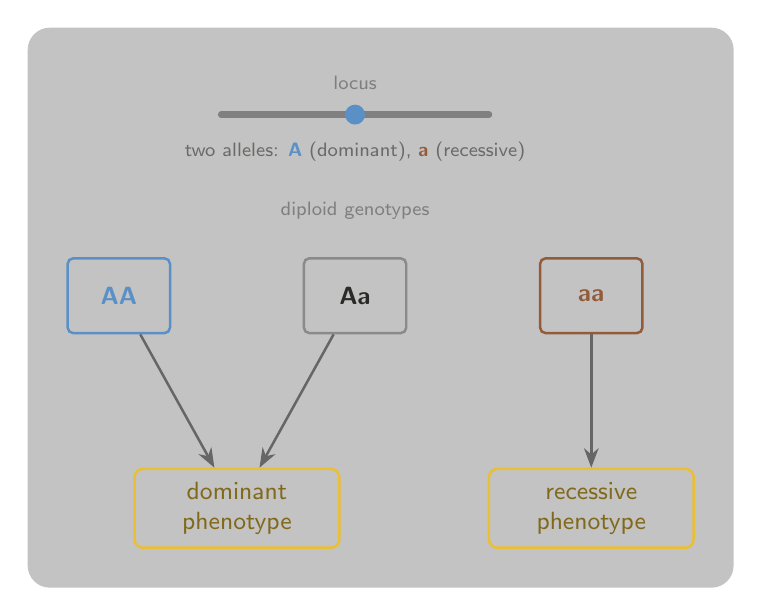
\begin{tikzpicture}[
    >=Stealth,
    font=\sffamily,
    lab/.style={font=\sffamily\scriptsize, text=gtbink!60, align=center},
    geno/.style={draw, rounded corners=2pt, line width=0.9pt, minimum width=1.3cm,
                 minimum height=0.95cm, font=\sffamily\small\bfseries},
    phenob/.style={draw=phen, rounded corners=3pt, line width=0.9pt, align=center,
                   minimum width=2.6cm, minimum height=1.0cm, font=\sffamily\small,
                   text=phen!55!black},
]

% locus on a chromosome
\draw[line width=2.4pt, black!50, line cap=round] (-1.7,5) -- (1.7,5);
\fill[alleleA] (0,5) circle (3.6pt);
\node[lab, anchor=south] at (0,5.2) {locus};
\node[lab, anchor=north, text=gtbink!70] at (0,4.78)
   {two alleles: \textcolor{alleleA}{\textbf{A}} (dominant),
    \textcolor{allelea}{\textbf{a}} (recessive)};

% diploid genotypes
\node[lab, anchor=south] at (0,3.55) {diploid genotypes};
\node[geno, draw=alleleA, text=alleleA] (AA) at (-3,2.7) {AA};
\node[geno, draw=gtbink!55]               (Aa) at (0,2.7)  {Aa};
\node[geno, draw=allelea, text=allelea] (aa) at (3,2.7)  {aa};

% phenotypes
\node[phenob] (P1) at (-1.5,0) {dominant\\ phenotype};
\node[phenob] (P2) at (3,0)    {recessive\\ phenotype};

\draw[->, line width=0.9pt, black!60] (AA) -- (P1);
\draw[->, line width=0.9pt, black!60] (Aa) -- (P1);
\draw[->, line width=0.9pt, black!60] (aa) -- (P2);

\end{tikzpicture}
\end{document}
